%% Springer Nature LaTeX template (sn-jnl)
\documentclass[pdflatex,sn-mathphys-num]{sn-jnl}
\usepackage{graphicx}
\usepackage{multirow}
\usepackage{amsmath,amssymb,amsfonts}
\usepackage{amsthm}
\usepackage{mathrsfs}
\usepackage[title]{appendix}
\usepackage{xcolor}
\usepackage{textcomp}
\usepackage{manyfoot}
\usepackage{booktabs}
\usepackage{algorithm}
\usepackage{algorithmicx}
\usepackage{algpseudocode}
\usepackage{rotating}
\usepackage{url}
\raggedbottom
\begin{document}
\title[Short-Term Network Latency Prediction]{Can Machine Learning Beat TCP's Estimator? Short-Term Network Latency Prediction from an End Host}
\author*[1]{\fnm{Sanskar} \sur{Gupta}}
\affil*[1]{\orgdiv{Department of Computer Science and Engineering}, \orgname{Manipal University Jaipur}, \orgaddress{\city{Jaipur}, \state{Rajasthan}, \country{India}}}
\abstract{Network latency changes from second to second, and predicting it a few seconds ahead helps applications choose servers, adapt video quality and set protocol timers. Transport protocols such as TCP already predict the next round-trip time (RTT) with an exponentially weighted moving average (EWMA). This paper asks whether machine learning can do better using only information an ordinary end host has. A measurement tool recorded the TCP handshake RTT from a laptop to 12 servers in eight regions every 5 seconds, for one hour on a home Wi-Fi network (8,640 probes) and for 15 minutes on a mobile hotspot (2,076 probes). Features were built from past measurements only, and eight predictors (persistence, moving average, EWMA, ridge regression, k-nearest neighbours, decision tree, Random Forest and gradient boosting) were evaluated with forward-chaining splits, so every model was trained on the past and tested on the future. On Wi-Fi, ridge regression achieved the lowest mean absolute error, 38.50 ms, 6.9\% lower than EWMA, a difference significant under both the Diebold--Mariano test and a Wilcoxon test across servers. On the noisier mobile hotspot, EWMA was best (92.24 ms) and every learned model was significantly worse, although Random Forest trained only on recent data beat it. Across both networks, ridge regression and EWMA shared the top Friedman rank, while gradient boosting, chosen in advance as the proposed model, ranked near the bottom. The results show that EWMA remains a strong default and that a light model gives only modest gains on stable paths.}
\keywords{Network latency, Round-trip time, Time-series prediction, Machine learning, TCP, Forward-chaining evaluation}
\maketitle
% =====================================================================
%  Section 1: Related Work - network latency prediction
% =====================================================================
\section{Related Work}\label{sec:related}

Latency, the time a packet needs to travel from one host to another and back, decides how responsive the internet feels. Video calls, online games, cloud applications and even web page loading slow down noticeably when the round-trip time (RTT) rises by a few tens of milliseconds. Predicting latency a few seconds ahead lets a system react before users notice: an application can pick a closer server, a video player can lower its quality early, and a transport protocol can set better timers. This section reviews more than thirty studies on how latency is measured, estimated and predicted. Fig.~\ref{fig:taxonomy} groups them into four families, Fig.~\ref{fig:timeline} places the most important ones in time, Table~\ref{tab:complexity} compares their cost, Table~\ref{tab:comparison} compares 22 studies side by side, and the section ends with the measurable gaps addressed in this paper.

\begin{figure}[t]
\centering
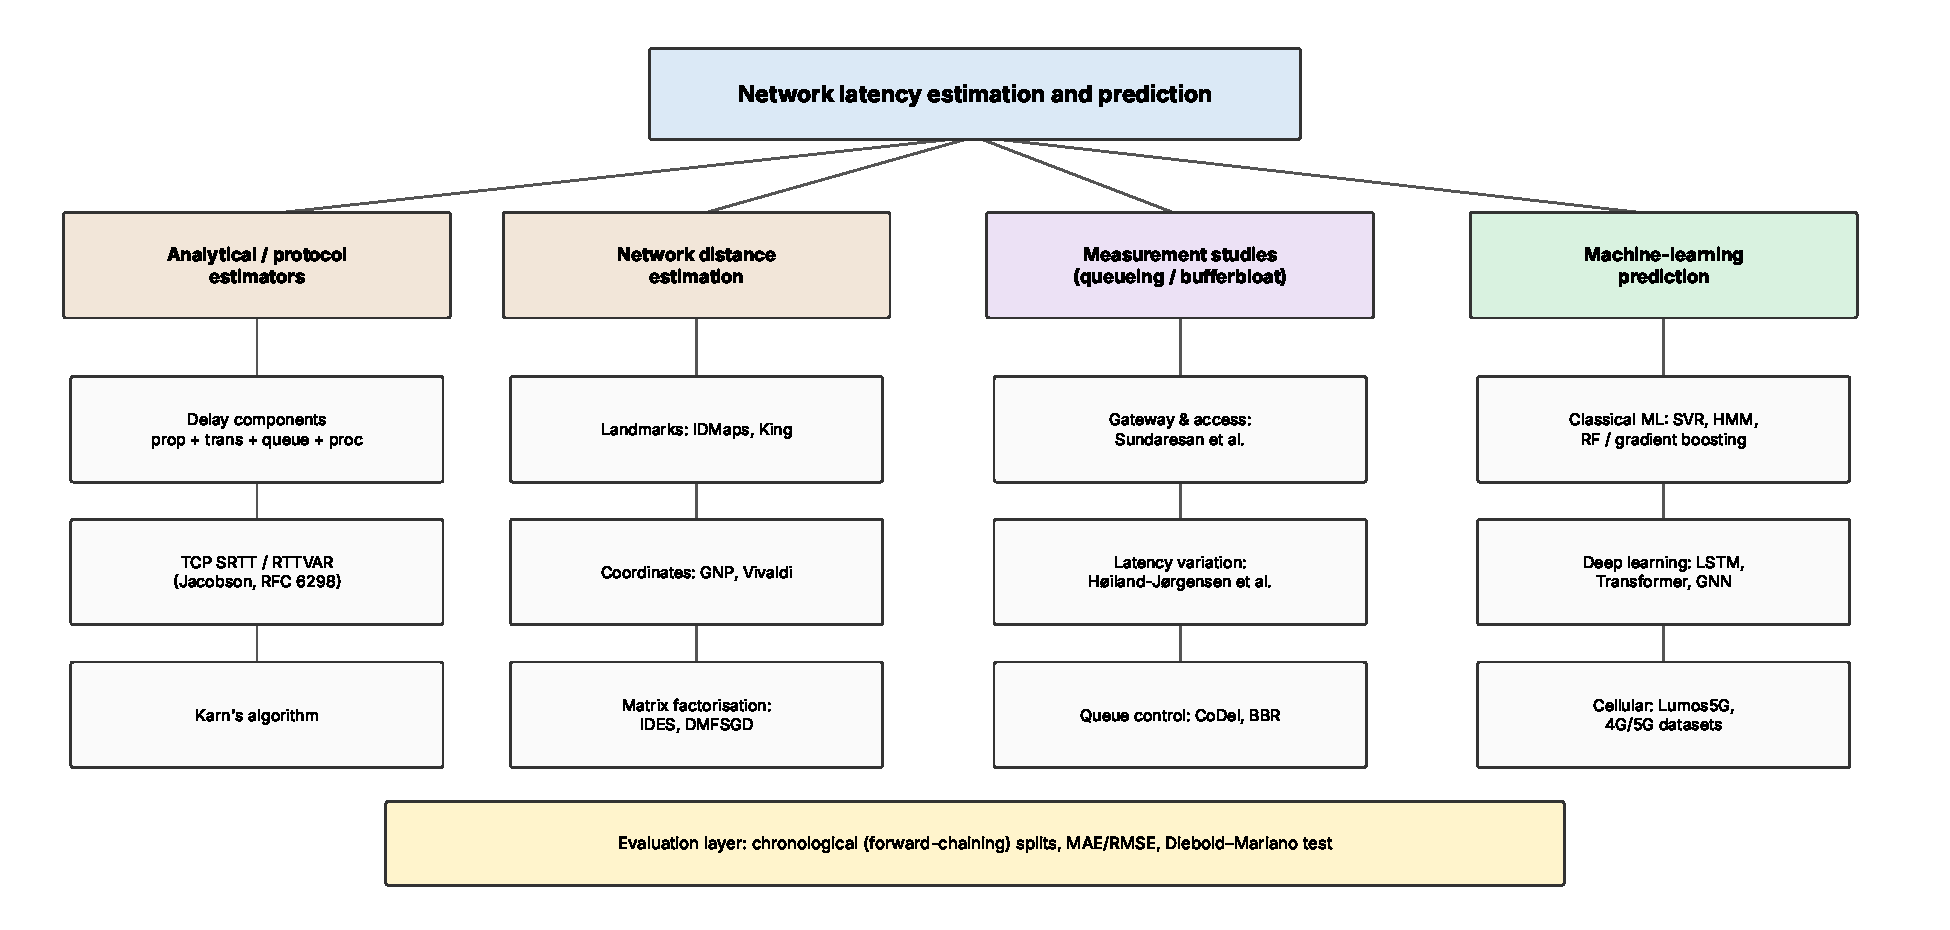
\includegraphics[width=\textwidth]{fig_taxonomy.pdf}
\caption{Families of approaches to network latency estimation and prediction}\label{fig:taxonomy}
\end{figure}

\subsection{What latency is made of}

Following the standard textbook view \cite{kurose2021}, the delay of a packet at each hop is the sum of four parts:
\begin{equation}
d_{\text{hop}} = d_{\text{proc}} + d_{\text{queue}} + d_{\text{trans}} + d_{\text{prop}}, \qquad
d_{\text{trans}} = \frac{L}{R}, \qquad d_{\text{prop}} = \frac{\ell}{v},
\label{eq:delay}
\end{equation}
where $d_{\text{proc}}$ is the time a router needs to process the packet header, $d_{\text{queue}}$ the time the packet waits in a buffer, $L$ the packet size in bits, $R$ the link rate, $\ell$ the length of the link and $v$ the signal speed in the medium (about $2\times10^8$ m/s in fibre). The RTT is the sum of these delays along the path to the destination and back. Propagation and transmission delay change only when the route or the link changes, so they set a floor on the RTT. Queueing delay, by contrast, changes from millisecond to millisecond with the amount of traffic. This is why RTT measured to the same server can double within seconds, and why short-term prediction is difficult.

Prediction is useful because many decisions in networked applications depend on latency in the near future rather than on its long-term average. A video player that expects the next chunk to arrive late can lower its quality before the buffer runs empty \cite{yan2020puffer,sun2016cs2p}; a client that can choose between several replicas of a service can send the next request to the one expected to answer fastest; and a transport protocol that sets its retransmission timer too low wastes bandwidth on needless retransmissions, while one that sets it too high reacts slowly to real losses \cite{rfc6298}. In each case, a better estimate of the next few seconds translates directly into a better user experience.

RTT is usually measured either with ICMP echo packets (ping) or by timing a TCP handshake: the client sends a SYN and measures how long the SYN/ACK takes to return. The second method uses the same packets real applications use and is not blocked by firewalls that drop ICMP, which is why it is used in this work.

\subsection{Classical RTT estimation in TCP}

TCP must estimate the RTT continuously to decide when a lost packet should be retransmitted. Jacobson's algorithm \cite{jacobson1988}, standardised in RFC 6298 \cite{rfc6298}, keeps an exponentially weighted moving average (EWMA) of RTT samples $R'$ and of their variation:
\begin{align}
\mathrm{RTTVAR} &\leftarrow (1-\beta)\,\mathrm{RTTVAR} + \beta\,\lvert \mathrm{SRTT} - R' \rvert, \label{eq:rttvar}\\
\mathrm{SRTT} &\leftarrow (1-\alpha)\,\mathrm{SRTT} + \alpha\,R', \label{eq:srtt}\\
\mathrm{RTO} &= \mathrm{SRTT} + 4\,\mathrm{RTTVAR}, \label{eq:rto}
\end{align}
with $\alpha = 1/8$ and $\beta = 1/4$. The smoothed RTT (SRTT) of Eq.~\ref{eq:srtt} is in effect a one-step-ahead prediction of the next RTT. Karn and Partridge \cite{karn1987} showed that RTT samples from retransmitted packets are ambiguous and must be ignored. These estimators are cheap and robust, but they only look at one connection's own past and cannot use outside information, such as whether the local link is busy. In this paper the EWMA of Eq.~\ref{eq:srtt}, together with simply repeating the last value (persistence) and a moving average, serves as a baseline that any machine-learning model must beat.

\subsection{Estimating latency between hosts}

A second line of work estimates the RTT between pairs of hosts without measuring every pair. IDMaps \cite{francis2001idmaps} placed measurement ``tracers'' in the network and estimated distances through them. King \cite{gummadi2002king} estimated the latency between two arbitrary hosts by timing recursive DNS queries between their nearby name servers. Coordinate systems went further. GNP \cite{ng2002gnp} measured each host's RTT to a few landmark hosts and placed every host in a geometric space, so that the distance between two points approximates their RTT. Vivaldi \cite{dabek2004vivaldi} removed the need for landmarks by treating each RTT as a spring between two nodes: node $i$ moves its coordinate $\mathbf{x}_i$ a small step $\delta$ along the error of each new measurement $\mathrm{rtt}_{ij}$,
\begin{equation}
\mathbf{x}_i \leftarrow \mathbf{x}_i + \delta\,\big(\mathrm{rtt}_{ij} - \lVert\mathbf{x}_i - \mathbf{x}_j\rVert\big)\,u(\mathbf{x}_i - \mathbf{x}_j),
\label{eq:vivaldi}
\end{equation}
where $u(\cdot)$ is a unit vector. On a set of 1{,}740 DNS servers, Vivaldi reached a median relative error of 11\% \cite{dabek2004vivaldi}. Because internet routes often violate the triangle inequality, later work replaced geometric embedding with low-rank matrix factorisation of the RTT matrix, $\hat{D} = XY^{\top}$: IDES \cite{mao2006ides} and the decentralised DMFSGD \cite{liao2012dmfsgd}, which reported a median absolute error of about 1 ms against about 5 ms for Vivaldi on one dataset. iPlane \cite{madhyastha2006iplane} predicted path properties by combining measured path segments. All of these methods estimate the \emph{typical} latency between hosts; none of them tries to predict how the latency will change in the next few seconds.

\subsection{Queueing delay and bufferbloat}

Measurement studies show why short-term changes matter. Sundaresan et al.~\cite{sundaresan2011broadband} measured home broadband from the gateway and found that latency under load can rise far above the idle value. Gettys and Nichols \cite{gettys2012bufferbloat} named this effect \emph{bufferbloat}: oversized buffers fill up during uploads or downloads and add hundreds of milliseconds of queueing delay. CoDel \cite{nichols2012codel} controls this delay inside routers, and BBR \cite{cardwell2017bbr} is a congestion-control algorithm that tries to keep queues short. Høiland-Jørgensen et al.~\cite{hoiland2016latency} analysed 265.8 million measurements and found that two thirds of them showed more than 100 ms of RTT variation, and that in access networks delay closely followed the amount of outbound traffic. These findings suggest that the state of the local link is a useful input for latency prediction, which this paper tests directly by switching a background download on and off during measurement.

\subsection{Machine learning for network performance prediction}

Machine learning has been widely applied in networking \cite{boutaba2018survey,mestres2017kdn}. Mirza et al.~\cite{mirza2007tcp} used support vector regression on simple path measurements, such as queueing delay and loss, to predict TCP throughput, and reached predictions within 10\% of the true value far more often than history-based predictors. CS2P \cite{sun2016cs2p} predicted video-session throughput with a hidden Markov model trained on similar sessions and cut median prediction error by 40--50\%. Puffer \cite{yan2020puffer} trained a neural network to predict how long the next video chunk would take to arrive and tested it in a randomised study with real users. In cellular networks, Lumos5G \cite{narayanan2020lumos5g} predicted mmWave 5G throughput from location and signal context and reduced prediction error by 1.37 to 4.84 times compared with earlier models, while Raca et al.\ released public 4G \cite{raca2018lte} and 5G \cite{raca2020nr} traces of channel and throughput metrics.

Fewer studies predict latency itself. Hagos et al.~\cite{hagos2019rtt} trained a long short-term memory (LSTM) network \cite{hochreiter1997lstm} to estimate TCP RTT from passive measurements in an emulated testbed and in the cloud, with mean absolute percentage errors mostly below about 2.6\%. Mostafavi et al.~\cite{mostafavi2025delay} forecast packet delay in a 5G testbed with LSTM and Transformer models that output a full probability distribution. RouteNet \cite{rusek2020routenet} used graph neural networks to predict per-path delay from the topology, routing and traffic matrix of a whole network, with a worst-case mean relative error of 15.4\% on unseen topologies; RouteNet-Fermi \cite{ferriol2023fermi} reduced this to 6.24\% on topologies about ten times larger than those seen in training. These models are accurate but need either a complete view of the network (RouteNet) or specialised radio and protocol information (5G testbeds), which a normal end host does not have.

\begin{figure}[t]
\centering
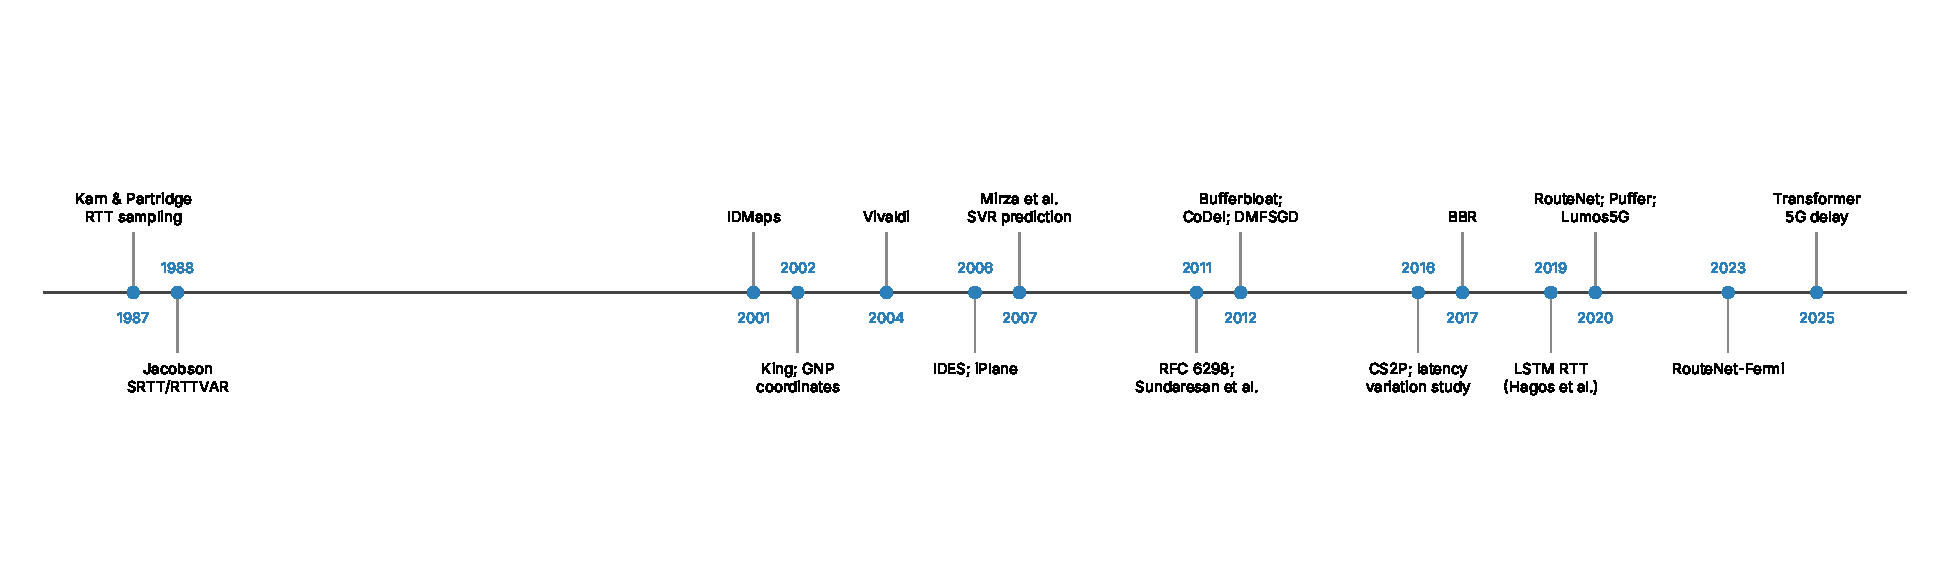
\includegraphics[width=\textwidth]{fig_timeline.pdf}
\caption{Timeline of important studies on latency estimation and prediction}\label{fig:timeline}
\end{figure}

\subsection{Learning methods and fair evaluation}

Tree ensembles are strong general-purpose regressors for tabular features. A Random Forest \cite{breiman2001rf} averages many decision trees trained on random samples, and gradient boosting \cite{friedman2001gbm} builds trees one after another, each fitting the remaining error of the previous ones:
\begin{equation}
F_m(\mathbf{x}) = F_{m-1}(\mathbf{x}) + \eta\, h_m(\mathbf{x}), \qquad
h_m = \arg\min_{h} \sum_{i} \big(r_{i}^{(m)} - h(\mathbf{x}_i)\big)^2,
\label{eq:gb}
\end{equation}
where $r_i^{(m)} = y_i - F_{m-1}(\mathbf{x}_i)$ is the residual of sample $i$ and $\eta$ is the learning rate. Histogram-based implementations such as LightGBM \cite{ke2017lightgbm} make this fast on large data. Classical time-series models such as ARIMA \cite{box2015arima} and recurrent networks such as LSTM \cite{hochreiter1997lstm} are the main alternatives.

How such models are tested matters as much as which model is chosen. In a time series, ordinary random cross-validation mixes past and future, so a model can be trained on measurements taken after the ones it is tested on. Bergmeir and Benítez \cite{bergmeir2012cv} and Cerqueira et al.~\cite{cerqueira2020eval} studied this problem and recommend evaluation schemes that respect time order, such as forward-chaining, where the model is always trained on the past and tested on the future. Hyndman and Koehler \cite{hyndman2006accuracy} discuss how to choose error measures, and the Diebold--Mariano test \cite{diebold1995dm} is the standard way to check whether one forecast is significantly more accurate than another.

\subsection{Computational cost}

Table~\ref{tab:complexity} compares the cost of the main technique families. Here $n$ is the number of training samples, $D$ the number of features, $B$ the number of trees, $N$ the number of hosts, $T$ the length of the input history and $H$ the hidden size of a neural network. The protocol estimators cost almost nothing, which is why TCP uses them. Tree ensembles need more work to train but predict in microseconds. Deep sequence models and graph neural networks are the most expensive and usually need a GPU.

\begin{table}[h]
\caption{Computational cost of common latency estimation and prediction techniques}\label{tab:complexity}
\centering
\footnotesize
\begin{tabular}{@{}p{3.3cm}p{3.3cm}p{2.6cm}p{3.4cm}@{}}
\toprule
Technique & Training / set-up cost & Cost per prediction & Remark \\
\midrule
Persistence / EWMA (TCP) \cite{rfc6298} & none & $O(1)$ & Uses only its own past \\
Coordinates (GNP, Vivaldi) \cite{ng2002gnp,dabek2004vivaldi} & $O(N)$ probes per round & $O(\text{dim})$ & Typical, not short-term, RTT \\
Matrix factorisation \cite{mao2006ides,liao2012dmfsgd} & $O(N r)$ per update & $O(r)$ & $r$ = rank; static distances \\
Ridge regression & $O(nD^2 + D^3)$ & $O(D)$ & Linear only \\
$k$-nearest neighbours & none & $O(nD)$ & Slow for large $n$ \\
Random Forest \cite{breiman2001rf} & $O(B\,n\sqrt{D}\log n)$ & $O(B\log n)$ & Parallel over trees \\
Gradient boosting \cite{friedman2001gbm,ke2017lightgbm} & $O(M\,n\,D)$ (histogram) & $O(M\cdot\text{depth})$ & $M$ sequential trees \\
LSTM \cite{hochreiter1997lstm,hagos2019rtt} & $O(E\,n\,T\,H^2)$ & $O(T\,H^2)$ & $E$ epochs; GPU \\
Graph neural network \cite{rusek2020routenet} & high (GPU, many topologies) & $O(\text{iterations}\times\text{paths})$ & Needs full network view \\
\botrule
\end{tabular}
\end{table}

\subsection{Comparison of existing studies}

Table~\ref{tab:comparison} compares 22 studies on seven parameters: year, goal, method, input data, scale of evaluation, best reported result and main limitation for short-term, end-host latency prediction. Results are copied from the original papers; ``n.r.'' means a value was not stated in the source reviewed.

\begin{sidewaystable}
\caption{Comparison of 22 studies on latency estimation and network performance prediction}\label{tab:comparison}
\centering
\scriptsize
\setlength{\tabcolsep}{3pt}
\begin{tabular}{@{}p{2.8cm}p{0.6cm}p{2.5cm}p{2.7cm}p{2.9cm}p{2.6cm}p{2.9cm}p{3.6cm}@{}}
\toprule
Study & Year & Goal & Method & Input data & Evaluation scale & Best reported result & Limitation for short-term prediction \\
\midrule
Karn \& Partridge \cite{karn1987} & 1987 & RTT sampling & Ignore retransmitted samples & TCP ACK timing & Analytical & Removes ambiguity & No prediction model \\
Jacobson \cite{jacobson1988}; RFC 6298 \cite{rfc6298} & 1988 & RTT estimate for timers & EWMA (SRTT, RTTVAR) & Own RTT samples & Standard in all TCP & n.r. & Uses only own past \\
Francis et al.\ (IDMaps) \cite{francis2001idmaps} & 2001 & Host distance & Tracer landmarks & Tracer RTTs & Internet-wide & n.r. & Static, coarse \\
Gummadi et al.\ (King) \cite{gummadi2002king} & 2002 & Host-pair RTT & Recursive DNS timing & DNS servers & Many host pairs & n.r. & Static estimate \\
Ng \& Zhang (GNP) \cite{ng2002gnp} & 2002 & Host distance & Landmark coordinates & Landmark RTTs & Internet hosts & More accurate than IDMaps & Needs landmarks; static \\
Dabek et al.\ (Vivaldi) \cite{dabek2004vivaldi} & 2004 & Host distance & Spring coordinates & Pairwise RTTs & 1,740 hosts & Median rel.\ error 11\% & Typical RTT only \\
Mao et al.\ (IDES) \cite{mao2006ides} & 2006 & Host distance & Matrix factorisation & Landmark RTTs & Large networks & n.r. & Static distances \\
Madhyastha et al.\ (iPlane) \cite{madhyastha2006iplane} & 2006 & Path properties & Path segment composition & Traceroutes & Internet-wide & n.r. & Heavy infrastructure \\
Mirza et al.\ \cite{mirza2007tcp} & 2007 & TCP throughput & SVR & Delay, loss, history & Lab + 18 paths & 87\% within 10\% (lab) & Throughput, not RTT \\
Sundaresan et al.\ \cite{sundaresan2011broadband} & 2011 & Broadband measurement & Gateway measurement & Home gateways & Many homes & Large delay under load & Measurement only \\
Gettys \& Nichols \cite{gettys2012bufferbloat} & 2012 & Explain excess delay & Analysis & Buffers & -- & Names bufferbloat & No prediction \\
Nichols \& Jacobson (CoDel) \cite{nichols2012codel} & 2012 & Control queue delay & Active queue management & Queue sojourn time & Routers & Short queues & Needs router change \\
Liao et al.\ (DMFSGD) \cite{liao2012dmfsgd} & 2012 & Host distance & Decentralised MF & Pairwise RTTs & Up to 2,500 nodes & Median AE $\approx$1 ms & Static distances \\
Sun et al.\ (CS2P) \cite{sun2016cs2p} & 2016 & Video throughput & HMM & Session features & Large video traces & 40--50\% lower error & Throughput, not RTT \\
H{\o}iland-J{\o}rgensen et al.\ \cite{hoiland2016latency} & 2016 & Latency variation & Measurement analysis & 265.8 M tests & Internet-wide & 2/3 samples $>$100 ms span & No prediction \\
Cardwell et al.\ (BBR) \cite{cardwell2017bbr} & 2017 & Congestion control & Model-based rate & Bandwidth, min RTT & Deployed at scale & n.r. & Not a predictor \\
Hagos et al.\ \cite{hagos2019rtt} & 2019 & TCP RTT & LSTM & Passive TCP traces & Testbed + cloud & MAPE $<$2.6\% & Emulated paths; GPU \\
Rusek et al.\ (RouteNet) \cite{rusek2020routenet} & 2020 & Path delay & Graph neural network & Topology, routing, traffic & Simulated networks & Worst MRE 15.4\% & Needs full network view \\
Yan et al.\ (Puffer) \cite{yan2020puffer} & 2020 & Chunk transfer time & Neural network & TCP statistics & Real users & Better video QoE & Video-specific \\
Narayanan et al.\ (Lumos5G) \cite{narayanan2020lumos5g} & 2020 & 5G throughput & ML (tree, seq.) & Location, signal & One city & 1.37--4.84$\times$ lower error & Throughput; 5G only \\
Ferriol-Galm{\'e}s et al.\ \cite{ferriol2023fermi} & 2023 & Path delay & Graph neural network & Topology, traffic & 10$\times$ larger nets & MRE 6.24\% & Needs full network view \\
Mostafavi et al.\ \cite{mostafavi2025delay} & 2025 & 5G packet delay & LSTM, Transformer & Radio + packet context & 5G testbed & Transformer best & Radio data; GPU \\
\botrule
\end{tabular}
\end{sidewaystable}

\subsection{Limitations of existing work}\label{sec:limitations}

Reading Table~\ref{tab:comparison} as a whole shows five gaps.
\begin{enumerate}
\item \textbf{Most methods estimate typical, not future, latency.} Seven of the 22 studies (IDMaps, King, GNP, Vivaldi, IDES, iPlane and DMFSGD) estimate a fixed distance between hosts. Even the best of them, with a median relative error of 11\% \cite{dabek2004vivaldi}, says nothing about the next few seconds, while measurements show that RTT varies by more than 100 ms in two thirds of samples \cite{hoiland2016latency}.
\item \textbf{Prediction work often targets throughput.} Of the eight machine-learning studies in the table, four (Mirza et al., CS2P, Puffer and Lumos5G) predict throughput or transfer time rather than RTT.
\item \textbf{The strongest delay models need information an end host lacks.} RouteNet and RouteNet-Fermi (MRE 15.4\% and 6.24\%) need the whole topology and traffic matrix, and the 5G delay models need radio-layer data \cite{rusek2020routenet,ferriol2023fermi,mostafavi2025delay}.
\item \textbf{Simple baselines are rarely the reference.} TCP already predicts the next RTT with an EWMA (Eq.~\ref{eq:srtt}). Apart from Hagos et al., who compare against TCP's own smoothed RTT \cite{hagos2019rtt}, the delay predictors in Table~\ref{tab:comparison} (RouteNet, RouteNet-Fermi and Mostafavi et al.) report, in the material reviewed here, comparisons with other learned or analytical models rather than with persistence or EWMA.
\item \textbf{Time-order and significance are rarely checked.} Hagos et al.\ used a 60/40 split with 5-fold cross-validation \cite{hagos2019rtt}; random folds on time-series data can place future samples in the training set \cite{bergmeir2012cv,cerqueira2020eval}. None of the ML studies in the table reports a forecast-comparison test such as Diebold--Mariano \cite{diebold1995dm}.
\end{enumerate}

This paper responds to these gaps. It predicts the next RTT of real servers from an ordinary laptop, using only information an end host has: the recent RTT history of each server, the RTTs of other servers and whether the local link is busy. It compares machine-learning models against the persistence, moving-average and EWMA estimators used by TCP, evaluates everything with forward-chaining splits so the model never sees the future, and tests significance with the Diebold--Mariano test.

% =====================================================================
%  Section 2: Proposed Work - latency prediction
% =====================================================================
\section{Proposed Work}\label{sec:proposed}

The gaps in Section~\ref{sec:limitations} lead to one practical question. Using only information that an ordinary end host has, can machine learning predict a server's next round-trip time better than the simple estimators TCP already uses? This section explains four things: how real latency data were collected, how features were built from past measurements only, which models were compared, and how they were tested without letting any model see the future. Fig.~\ref{fig:methodology} shows the full pipeline.

\begin{figure}[t]
\centering
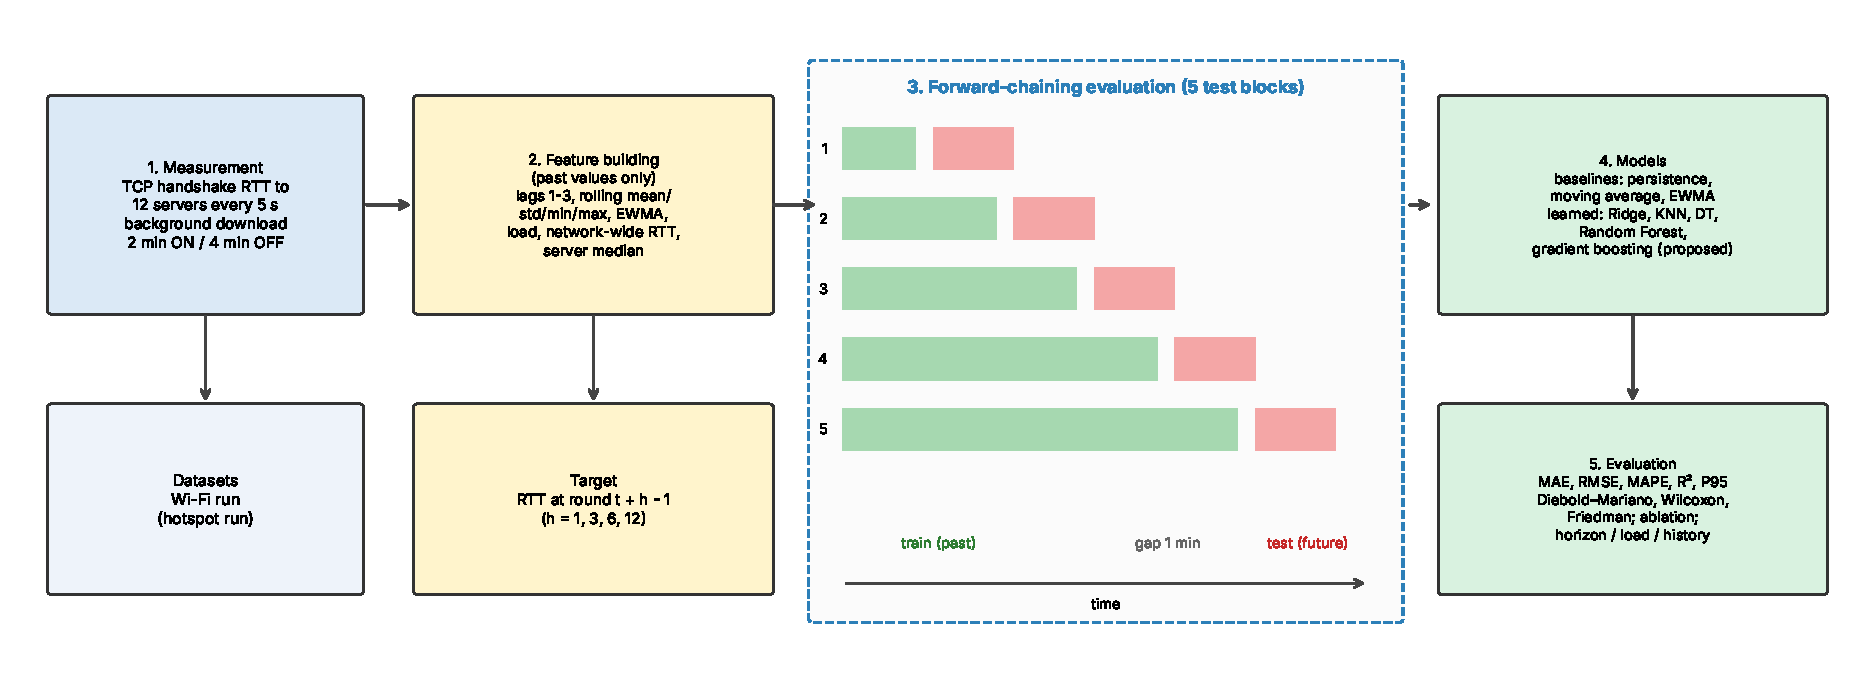
\includegraphics[width=\textwidth]{fig_methodology.pdf}
\caption{Proposed pipeline: RTT measurement, feature building from past values only, forward-chaining evaluation in which every model is trained on the past and tested on the future, and comparison of learned models with classical estimators}\label{fig:methodology}
\end{figure}

\subsection{Methodology}\label{sec:method}

\textbf{Stage 1: Measurement.} A Python program running on a laptop measured the RTT to 12 public web servers chosen to cover different regions and network types: global content delivery networks (Google, Cloudflare, Wikipedia, GitHub), servers in India (Amazon India, Manipal University) and servers in the United States, United Kingdom, Japan, Australia, Brazil and South Africa. Each server's domain name was resolved once at the start, so DNS lookup time is not mixed into the measurements. Every 5 seconds, the program opened a TCP connection to port 443 of each server. It recorded the time between sending the SYN and receiving the SYN/ACK. This time is one RTT plus a very small processing time. A probe that did not finish within 3 seconds was recorded as a failure. In the Wi-Fi run, a background download was also switched on for 2 minutes in every 6-minute cycle, to create both quiet and busy periods. While the download runs, the local link is busy and queueing delay (Eq.~\ref{eq:delay}) should increase, as described in the bufferbloat literature \cite{gettys2012bufferbloat,hoiland2016latency}. One round of probes to all 12 servers is called a \emph{round}.

\textbf{Stage 2: Feature building.} For every server and every round $t$, a feature vector is built using \emph{only measurements from rounds before $t$}, so that the model has exactly the information it would have in real time. The features fall into four groups. \emph{Lag} features are the server's last three RTTs. \emph{Rolling} features describe its recent behaviour: the mean, standard deviation, minimum and maximum of the last 5 RTTs; the mean and standard deviation of the last 12 RTTs (one minute); an EWMA with $\lambda = 0.3$; and the last change in RTT. \emph{Context} features describe the network as a whole: whether the background download is running, the mean and standard deviation of all servers' RTTs in the previous round, and the share of failed probes to this server in the last minute. \emph{Server} features are the server's median RTT so far and an identifier. The value to be predicted is the server's RTT $h$ rounds ahead, where $h = 1$ (the next 5 seconds) in the main experiment. If a probe failed, its RTT is not used as a target, and the last valid value is carried forward when building features.

\textbf{Stage 3: Models.} Three classical estimators that need no training are used as baselines: \emph{persistence} (the next RTT equals the last one), a 5-sample \emph{moving average} and an \emph{EWMA}, the same kind of estimator TCP uses (Eq.~\ref{eq:srtt}). Five learned regressors are compared with them: ridge regression, $k$-nearest neighbours ($k = 10$), a decision tree, a Random Forest with 200 trees \cite{breiman2001rf} and histogram-based gradient boosting \cite{friedman2001gbm,ke2017lightgbm}. Gradient boosting was chosen in advance as the proposed model for two reasons. It can learn non-linear interactions between features, such as a busy link that only matters for distant servers. It is also cheap enough to retrain on an end host. All models use scikit-learn \cite{pedregosa2011sklearn}, and scaling for ridge regression and $k$-nearest neighbours is fitted on training data only.

\textbf{Stage 4: Forward-chaining evaluation.} The rounds are kept in time order. The first 40\% of rounds form the initial training history, and the remaining rounds are divided into five consecutive test blocks. For test block $i$, every model is trained on all rounds before that block and then tested on the block. The last 12 rounds (one minute) before the block are left out as a gap, so that rolling windows in the test block cannot overlap with training targets. In simple terms, the model is always trained on the past and tested on the future, just as it would be used in real life. Random cross-validation would mix past and future rows, so this design is recommended for time series instead \cite{bergmeir2012cv,cerqueira2020eval}.

\subsection{Mathematical model}\label{sec:model}

Let $y_{s,t}$ be the RTT of server $s$ in round $t$, and let $\mathcal{H}_{s,t} = \{y_{s',t'} : t' < t\}$ be everything measured before round $t$. The feature vector $\mathbf{x}_{s,t} = \phi(\mathcal{H}_{s,t}, \ell_t)$ is built from this history and the current load indicator $\ell_t \in \{0,1\}$. For example, the rolling mean and standard deviation over the last $w$ rounds are
\begin{equation}
\mu^{(w)}_{s,t} = \frac{1}{w}\sum_{j=1}^{w} y_{s,t-j}, \qquad
\sigma^{(w)}_{s,t} = \sqrt{\frac{1}{w-1}\sum_{j=1}^{w}\big(y_{s,t-j} - \mu^{(w)}_{s,t}\big)^2},
\label{eq:rolling}
\end{equation}
In words, $\mu^{(w)}$ is the average RTT of the last $w$ rounds, and $\sigma^{(w)}$ shows how much the RTT has been jumping around (the recent jitter). The three baselines predict
\begin{equation}
\hat{y}^{\text{pers}}_{s,t} = y_{s,t-1}, \qquad
\hat{y}^{\text{MA}}_{s,t} = \mu^{(5)}_{s,t}, \qquad
\hat{y}^{\text{EWMA}}_{s,t} = e_{s,t}, \quad e_{s,t} = (1-\lambda)\,e_{s,t-1} + \lambda\, y_{s,t-1},
\label{eq:baselines}
\end{equation}
with $\lambda = 0.3$. Persistence simply repeats the last RTT, the moving average uses the mean of the last five, and EWMA gives 30\% weight to the newest RTT and 70\% to its previous estimate, so it smooths out short spikes. A learned model $f_\theta$ predicts $\hat{y}_{s,t+h-1} = f_\theta(\mathbf{x}_{s,t})$, with its parameters chosen on the training set $\mathcal{T}_i$ of test block $i$ by minimising the squared error
\begin{equation}
\theta_i = \arg\min_{\theta} \sum_{(s,t) \in \mathcal{T}_i} \big(y_{s,t+h-1} - f_\theta(\mathbf{x}_{s,t})\big)^2.
\label{eq:objective}
\end{equation}
Gradient boosting minimises Eq.~\ref{eq:objective} by adding trees one at a time as in Eq.~\ref{eq:gb}, with learning rate $\eta = 0.05$ and up to 300 trees. With $K = 5$ test blocks $\mathcal{B}_i$ and a gap of $g = 12$ rounds, the training set for block $i$ is
\begin{equation}
\mathcal{T}_i = \{(s,t) : t < \min(\mathcal{B}_i) - g\},
\label{eq:split}
\end{equation}
so every training example comes strictly before the test block. Eq.~\ref{eq:objective} means that each learned model is tuned to make its squared prediction errors on the past as small as possible, and Eq.~\ref{eq:split} guarantees that this past never includes the test period.

\subsection{Algorithm}\label{sec:algorithm}

Algorithm~\ref{alg:latency} summarises the procedure for one dataset.

\begin{algorithm}[t]
\caption{Leak-free short-term RTT prediction with forward-chaining evaluation}\label{alg:latency}
\begin{algorithmic}[1]
\Require Probe log of RTTs per server and round; horizon $h$; test blocks $K$; gap $g$
\Ensure Error metrics of every model on every test block
\For{each server $s$}
  \State Carry the last valid RTT forward over failed probes (past values only)
  \For{each round $t$}
    \State Build $\mathbf{x}_{s,t}$ from rounds $< t$ with Eq.~\ref{eq:rolling} and the load flag $\ell_t$
    \State Set the target $y_{s,t+h-1}$; drop the example if that probe failed
  \EndFor
\EndFor
\State Sort rounds in time order; keep the first 40\% as initial history; split the rest into $K$ blocks
\For{each test block $\mathcal{B}_i$, $i = 1, \dots, K$}
  \State $\mathcal{T}_i \gets$ all examples before $\min(\mathcal{B}_i) - g$ \Comment{Eq.~\ref{eq:split}}
  \State Compute the three baseline predictions with Eq.~\ref{eq:baselines}
  \For{each learned model}
    \State Fit on $\mathcal{T}_i$ by minimising Eq.~\ref{eq:objective}; predict every example in $\mathcal{B}_i$
  \EndFor
  \State Record MAE, RMSE, MAPE, $R^2$ and the 95th-percentile error for every model
\EndFor
\State \Return the mean and standard deviation of every metric over the $K$ blocks
\end{algorithmic}
\end{algorithm}

Table~\ref{tab:hyper} lists all settings. A fixed random seed (42) makes the learned models reproducible.

\begin{table}[h]
\caption{Settings of the measurement and the prediction experiment}\label{tab:hyper}
\centering
\footnotesize
\begin{tabular}{@{}lll@{}}
\toprule
Part & Setting & Value \\
\midrule
Measurement & Servers / probe interval / timeout & 12 / 5 s / 3 s \\
 & RTT method & TCP SYN to SYN/ACK, port 443 \\
 & Background load & 50 MB download loop, 2 min ON per 6 min \\
Features & Lags / rolling windows / EWMA $\lambda$ & 3 / 5 and 12 rounds / 0.3 \\
Models & Random Forest & 200 trees, min.\ 5 samples per leaf \\
 & Gradient boosting (proposed) & up to 300 trees, learning rate 0.05 \\
 & Ridge / $k$-NN / decision tree & $\alpha = 1$ / $k = 10$ / min.\ 20 per leaf \\
Evaluation & Test blocks / initial history / gap & 5 / 40\% / 12 rounds (1 min) \\
 & Horizons $h$ & 1, 3, 6, 12 rounds (5--60 s) \\
 & Random seed & 42 \\
\botrule
\end{tabular}
\end{table}

\subsection{Datasets}\label{sec:datasets}

Two datasets were collected for this study with the procedure of Stage 1 (Table~\ref{tab:datasets}), both on 11 October 2026 from the same laptop in India. The \emph{Wi-Fi} dataset was measured on a home Wi-Fi network for 60 minutes (18:59--19:59), producing 720 rounds and 8{,}640 probes, of which only 0.12\% failed. The \emph{hotspot} dataset was measured through a mobile phone hotspot for 15 minutes (22:37--22:52), producing 173 rounds and 2{,}076 probes with no failures; to save mobile data, the background download was not used in this run. The mobile network was slower and much noisier: its median RTT was 142.1 ms against 100.5 ms on Wi-Fi, and its 95th-percentile RTT was 612.2 ms against 411.7 ms. Table~\ref{tab:servers} shows how different the 12 servers are: median RTTs range from about 32 ms (Cloudflare and Amazon India, served from nearby data centres) to about 400 ms (servers in Brazil and South Africa), and the standard deviation ranges from 36 ms to 191 ms. Each server can therefore be seen as a separate latency time series with its own level and noise, which lets the experiment test prediction across very different paths.

\begin{table}[h]
\caption{The two collected latency datasets}\label{tab:datasets}
\centering
\footnotesize
\setlength{\tabcolsep}{3pt}
\begin{tabular}{@{}lccccccc@{}}
\toprule
Network & Duration & Rounds & Probes & Failed & Median RTT & 95th pct.\ RTT & Median RTT, load on / off \\
\midrule
Home Wi-Fi & 60 min & 720 & 8{,}640 & 0.12\% & 100.5 ms & 411.7 ms & 99.5 / 101.1 ms \\
Mobile hotspot & 15 min & 173 & 2{,}076 & 0.00\% & 142.1 ms & 612.2 ms & -- / 142.1 ms \\
\botrule
\end{tabular}
\end{table}

\begin{table}[h]
\caption{RTT statistics of the 12 servers (Wi-Fi dataset, successful probes)}\label{tab:servers}
\centering
\footnotesize
\begin{tabular}{@{}llrrrr@{}}
\toprule
Server & Region & Median (ms) & 95th pct.\ (ms) & Std.\ dev.\ (ms) & Success (\%) \\
\midrule
cloudflare.com & Global CDN & 32.1 & 116.6 & 50.3 & 100.0 \\
amazon.in & India & 32.9 & 115.5 & 73.4 & 100.0 \\
google.com & Global CDN & 45.5 & 152.6 & 53.8 & 99.9 \\
abc.net.au & Australia & 55.8 & 130.3 & 57.2 & 100.0 \\
manipal.edu & India & 68.5 & 145.2 & 47.2 & 100.0 \\
mit.edu & USA & 93.8 & 182.2 & 43.1 & 100.0 \\
bbc.co.uk & UK & 98.6 & 167.5 & 35.6 & 100.0 \\
github.com & USA/Global & 99.1 & 175.8 & 54.4 & 99.9 \\
wikipedia.org & Global CDN & 130.5 & 217.4 & 93.3 & 100.0 \\
yahoo.co.jp & Japan & 197.9 & 286.3 & 55.5 & 99.9 \\
uct.ac.za & South Africa & 390.4 & 455.7 & 80.8 & 100.0 \\
gov.br & Brazil & 399.2 & 512.2 & 190.9 & 99.0 \\
\botrule
\end{tabular}
\end{table}

On the hotspot, the server medians were also much closer together (about 102--135 ms for all but the three most distant servers), because the mobile access link added a large delay to every path. One observation from Table~\ref{tab:datasets} matters for the interpretation of the Wi-Fi results: the median RTT with the background download switched on (99.5 ms) was almost the same as with it off (101.1 ms). Either the home link had enough spare capacity, or the download did not run at full speed; the collector did not record the downloaded volume, so this cannot be decided from the data. The load flag is therefore kept as a feature, but the experiment cannot claim to have measured heavy congestion.

% =====================================================================
%  Section 3: Results - all numbers generated from results_both/*.csv
% =====================================================================
\section{Results and Discussion}\label{sec:results}

This section reports the results on both datasets (Table~\ref{tab:datasets}) with the settings in Table~\ref{tab:hyper}. The analysis used Python with scikit-learn \cite{pedregosa2011sklearn}. On each dataset every model was trained and tested on the same five forward-chaining blocks (Wi-Fi: 3{,}248 to 7{,}322 training and about 1{,}020 test examples per block; hotspot: about 800 to 1{,}770 training and 200 test examples), so all comparisons are paired.

\subsection{Evaluation parameters}\label{sec:metrics}

For $n$ test examples with measured RTT $y_i$ and prediction $\hat{y}_i$, the following parameters are computed:
\begin{align}
\mathrm{MAE} &= \frac{1}{n}\sum_{i=1}^{n} \lvert y_i - \hat{y}_i \rvert, \qquad
\mathrm{RMSE} = \sqrt{\frac{1}{n}\sum_{i=1}^{n} (y_i - \hat{y}_i)^2}, \label{eq:mae}\\
\mathrm{MAPE} &= \frac{100\%}{n}\sum_{i=1}^{n} \frac{\lvert y_i - \hat{y}_i \rvert}{y_i}, \qquad
R^2 = 1 - \frac{\sum_i (y_i - \hat{y}_i)^2}{\sum_i (y_i - \bar{y})^2}. \label{eq:r2}
\end{align}
MAE (Eq.~\ref{eq:mae}) is the average error in milliseconds. It is the main measure because it is easy to understand and is not dominated by a few extreme spikes. RMSE squares the errors, so it punishes large errors more. MAPE gives the error as a percentage of the RTT, which makes fast and slow servers comparable. $R^2$ (Eq.~\ref{eq:r2}) is the share of RTT variation that the model explains: 1 is perfect, and 0 or below means the model is no better than always predicting the average \cite{hyndman2006accuracy}. The 95th-percentile absolute error (P95) shows how bad the worst predictions are.

To check whether one model is really more accurate than another, two tests were used. The \emph{Diebold--Mariano} (DM) test \cite{diebold1995dm} compares the absolute errors of two models. Because errors in consecutive rounds are correlated, the difference in absolute error $d_t$ is first averaged over the 12 servers in each round $t$, and its variance is estimated with 12 lags (one minute):
\begin{equation}
\mathrm{DM} = \frac{\bar{d}}{\sqrt{\frac{1}{T}\left(\hat{\gamma}_0 + 2\sum_{k=1}^{12}\hat{\gamma}_k\right)}},
\label{eq:dm}
\end{equation}
where $\bar{d}$ is the mean difference over $T$ test rounds and $\hat{\gamma}_k$ is its autocovariance at lag $k$. Put simply, DM checks whether the average gap between two models' errors is large compared with its normal random variation. A negative value means the first model has the smaller error. The \emph{Wilcoxon signed-rank test} \cite{wilcoxon1945} compares the two models' MAE across the 12 servers, which are independent paths. All $p$-values are adjusted with the Holm method \cite{holm1979}. The Friedman test \cite{friedman1937,demsar2006stat} ranks all eight models on each server of each dataset (24 blocks).

\subsection{Overview of the measured latency}

Fig.~\ref{fig:rtt} shows the RTT distribution of each server. The servers fall into three groups: nearby content delivery networks and Indian servers (median 32--69 ms), servers in Australia, the United States, the United Kingdom and Wikipedia's edge (56--131 ms), and distant servers in Japan, South Africa and Brazil (198--399 ms). Even nearby servers showed occasional spikes of several hundred milliseconds. On the mobile hotspot every RTT was higher (median 142 ms) and far more variable, with spikes above 1{,}000 ms on most servers.

\begin{figure}[h]
\centering
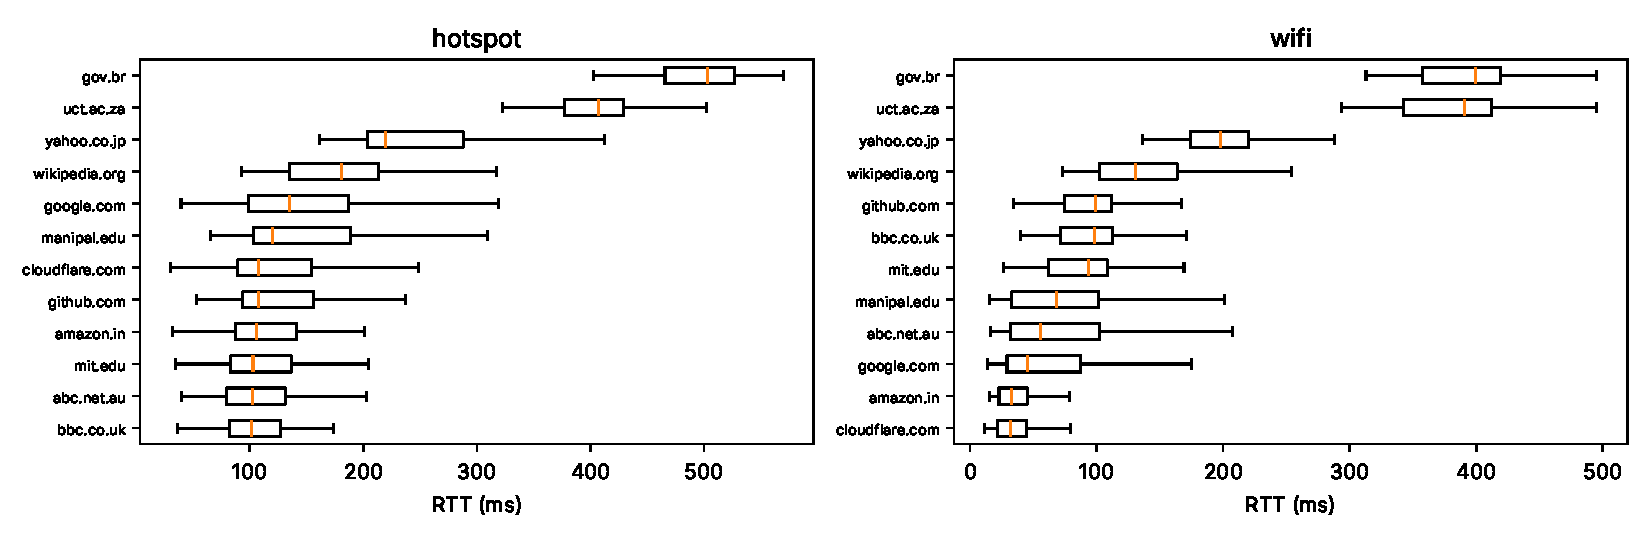
\includegraphics[width=\textwidth]{fig_rtt_servers.pdf}
\caption{RTT distribution of the 12 servers on the mobile hotspot (left) and the Wi-Fi network (right); boxes show the middle 50\% of values}\label{fig:rtt}
\end{figure}

\subsection{Comparison of prediction models}\label{sec:main_results}

Table~\ref{tab:main} and Fig.~\ref{fig:mae} compare the eight models for predicting the RTT 5 seconds ahead.

\begin{table}[h]
\caption{One-step-ahead (5 s) RTT prediction on both datasets (mean $\pm$ sd over 5 forward-chaining test blocks; MAE, RMSE and P95 in ms)}\label{tab:main}
\centering
\footnotesize
\begin{tabular}{@{}lcccccc@{}}
\toprule
Model & MAE & RMSE & MAPE (\%) & $R^2$ & P95 error & Fit time (s) \\
\midrule
\multicolumn{7}{@{}l}{\textit{Wi-Fi}}\\
Persistence & 50.61 $\pm$ 2.55 & 104.04 $\pm$ 37.13 & 60.95 & 0.50 & 128.21 & 0.00 \\
MovingAvg5 & 42.32 $\pm$ 3.84 & 83.15 $\pm$ 32.35 & 52.42 & 0.68 & 105.31 & 0.00 \\
EWMA & 41.37 $\pm$ 3.45 & 81.12 $\pm$ 30.22 & 51.44 & 0.69 & 104.83 & 0.00 \\
Ridge & \textbf{38.50} $\pm$ 2.29 & 77.35 $\pm$ 28.04 & 47.09 & 0.72 & 103.91 & 0.01 \\
KNN & 41.80 $\pm$ 3.71 & 81.65 $\pm$ 28.37 & 51.87 & 0.69 & 117.44 & 0.00 \\
DT & 44.67 $\pm$ 2.98 & 83.03 $\pm$ 28.29 & 55.21 & 0.68 & 120.25 & 0.07 \\
RF & 41.57 $\pm$ 3.99 & 80.11 $\pm$ 29.31 & 53.44 & 0.70 & 114.54 & 5.31 \\
GB (proposed) & 44.56 $\pm$ 3.60 & 86.86 $\pm$ 29.94 & 54.51 & 0.65 & 121.11 & 0.90 \\
\midrule
\multicolumn{7}{@{}l}{\textit{Mobile hotspot}}\\
Persistence & 110.09 $\pm$ 61.42 & 223.25 & 68.14 & -0.05 & 378.73 & 0.00 \\
MovingAvg5 & 96.04 $\pm$ 53.89 & 172.90 & 57.30 & 0.38 & 310.57 & 0.00 \\
EWMA & \textbf{92.24} $\pm$ 51.93 & 169.41 & 54.85 & 0.41 & 304.82 & 0.00 \\
Ridge & 102.73 $\pm$ 47.74 & 173.63 & 60.10 & 0.37 & 305.77 & 0.03 \\
KNN & 103.67 $\pm$ 57.18 & 184.56 & 61.95 & 0.30 & 340.31 & 0.00 \\
DT & 121.90 $\pm$ 56.44 & 202.32 & 77.70 & 0.13 & 413.32 & 0.01 \\
RF & 108.21 $\pm$ 56.12 & 181.57 & 72.41 & 0.32 & 351.77 & 0.77 \\
GB (proposed) & 139.79 $\pm$ 71.04 & 234.50 & 95.41 & -0.15 & 541.56 & 0.70 \\
\botrule
\end{tabular}
\end{table}

\begin{figure}[h]
\centering
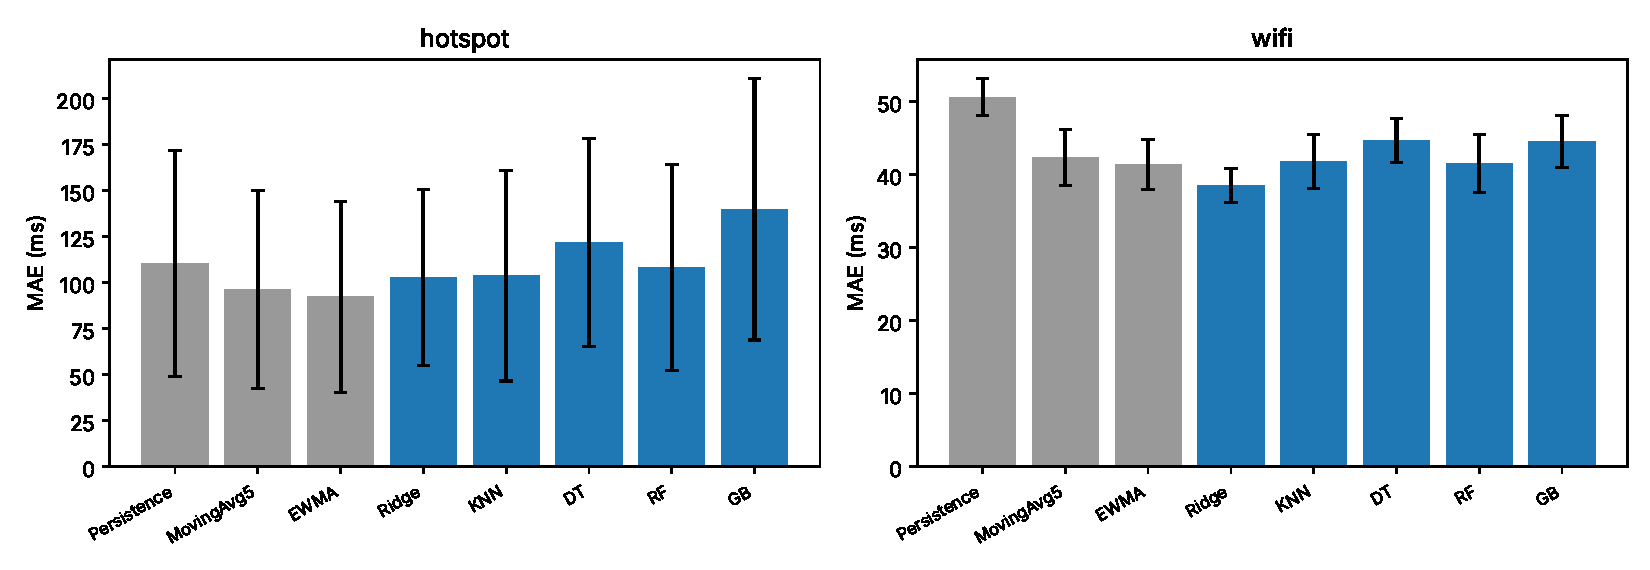
\includegraphics[width=\textwidth]{fig_mae_models.pdf}
\caption{MAE of each model on the mobile hotspot (left) and Wi-Fi (right) (grey: classical estimators without training; blue: learned models). Error bars show the standard deviation over the five test blocks}\label{fig:mae}
\end{figure}

On Wi-Fi, three findings stand out. First, simply repeating the last RTT (persistence) was the worst method, with an MAE of 50.61 ms, while the EWMA used in TCP reduced it to 41.37 ms. Smoothing therefore removes much of the random jitter. Second, ridge regression was the most accurate model, with an MAE of 38.50 ms, 6.9\% lower than EWMA, and also the best RMSE (77.35 ms) and $R^2$ (0.72). Third, the more complex models did not help. Random Forest (41.57 ms) and $k$-nearest neighbours (41.80 ms) were about as accurate as EWMA, and gradient boosting, which was chosen in advance as the proposed model, reached only 44.56 ms, 7.7\% worse than EWMA. All MAPE values were high (47--61\%) because many servers have low median RTTs, so even small absolute errors are large in relative terms, and occasional spikes of several hundred milliseconds are impossible to foresee. Fig.~\ref{fig:trace} illustrates this on one server: a spike to over 1{,}000 ms was missed by every model, and afterwards EWMA stayed too high for about 40 seconds, while gradient boosting returned to normal almost at once.

The mobile hotspot gave a different ranking. Errors were more than twice as large, and EWMA was the most accurate method (MAE 92.24 ms, $R^2 = 0.41$), followed by the moving average (96.04 ms). Every learned model was worse than EWMA: ridge regression by 11\%, Random Forest by 17\% and gradient boosting by 51\%, whose negative $R^2$ means it was less accurate than predicting the mean.

\begin{figure}[h]
\centering
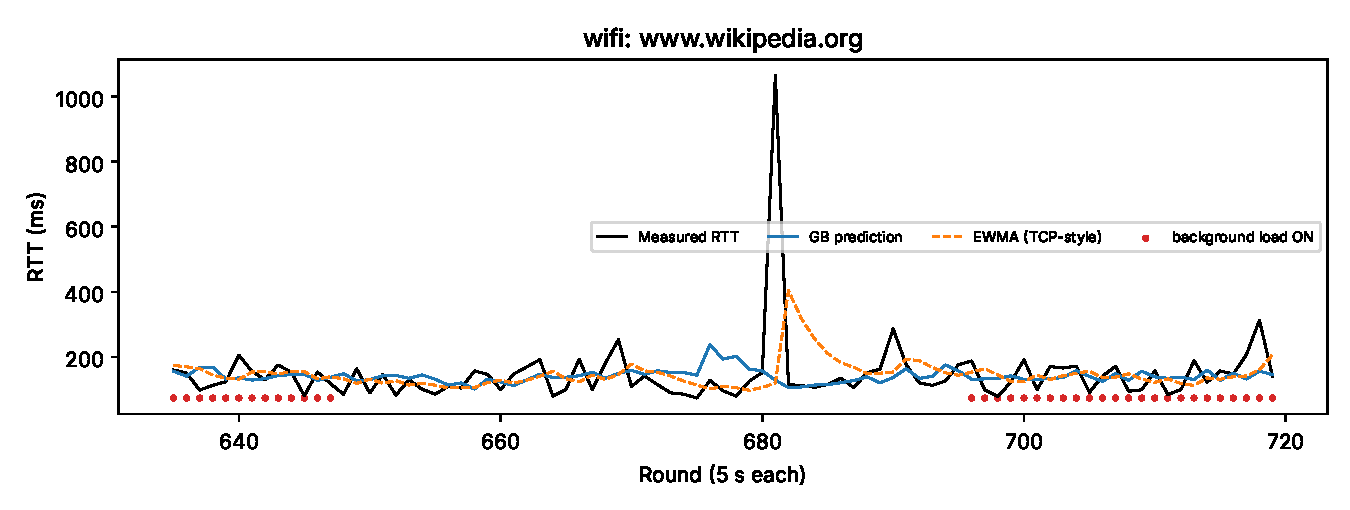
\includegraphics[width=\textwidth]{fig_trace_wifi.pdf}
\caption{Measured RTT and predictions for one server during the last test block. Red dots mark rounds with the background download switched on}\label{fig:trace}
\end{figure}

The cost of the models also differs widely: ridge regression trains in a few hundredths of a second and the classical estimators need no training, while Random Forest needs up to 5 seconds per block (Table~\ref{tab:main}). All models predict in under a millisecond, so all of them could run on an end host.

\subsection{Statistical tests}\label{sec:stats}

Table~\ref{tab:stats} reports the pairwise tests. A negative DM statistic and a positive MAE reduction mean that the first model in the row was more accurate.

\begin{table}[h]
\caption{Pairwise comparisons: MAE (ms) of the two models, MAE reduction of model A relative to B, DM statistic, and Holm-adjusted $p$-values of the DM test and of the Wilcoxon test over 12 servers ($^{*}$ adjusted $p < 0.05$)}\label{tab:stats}
\centering
\footnotesize
\begin{tabular}{@{}lcccccc@{}}
\toprule
A vs B & MAE A & MAE B & Reduction (\%) & DM & $p_{\mathrm{DM}}$ & $p_{\mathrm{Wilcoxon}}$ \\
\midrule
\multicolumn{7}{@{}l}{\textit{Wi-Fi}}\\
GB vs Persistence & 44.56 & 50.61 & +12.0 & -3.35 & 0.007$^{*}$ & 0.308 \\
GB vs Moving avg. & 44.56 & 42.32 & -5.3 & 1.47 & 0.570 & 1.000 \\
GB vs EWMA & 44.56 & 41.37 & -7.7 & 2.21 & 0.137 & 1.000 \\
GB vs Ridge & 44.56 & 38.50 & -15.7 & 7.88 & $<$0.001$^{*}$ & 0.038$^{*}$ \\
GB vs KNN & 44.56 & 41.80 & -6.6 & 2.66 & 0.047$^{*}$ & 1.000 \\
GB vs DT & 44.56 & 44.67 & +0.3 & -0.15 & 1.000 & 0.776 \\
GB vs RF & 44.56 & 41.56 & -7.2 & 3.57 & 0.004$^{*}$ & 0.308 \\
Ridge vs EWMA & 38.50 & 41.37 & +6.9 & -3.21 & 0.009$^{*}$ & 0.049$^{*}$ \\
KNN vs EWMA & 41.80 & 41.37 & -1.0 & 0.47 & 1.000 & 1.000 \\
DT vs EWMA & 44.67 & 41.37 & -8.0 & 3.25 & 0.009$^{*}$ & 0.308 \\
RF vs EWMA & 41.56 & 41.37 & -0.5 & 0.20 & 1.000 & 1.000 \\
\midrule
\multicolumn{7}{@{}l}{\textit{Mobile hotspot}}\\
GB vs Persistence & 141.21 & 111.73 & -26.4 & 3.79 & $<$0.001$^{*}$ & 0.034$^{*}$ \\
GB vs Moving avg. & 141.21 & 97.36 & -45.0 & 5.06 & $<$0.001$^{*}$ & 0.005$^{*}$ \\
GB vs EWMA & 141.21 & 93.55 & -51.0 & 5.31 & $<$0.001$^{*}$ & 0.005$^{*}$ \\
GB vs Ridge & 141.21 & 103.97 & -35.8 & 3.38 & 0.003$^{*}$ & 0.005$^{*}$ \\
GB vs KNN & 141.21 & 105.35 & -34.0 & 3.48 & 0.003$^{*}$ & 0.005$^{*}$ \\
GB vs DT & 141.21 & 123.02 & -14.8 & 3.01 & 0.008$^{*}$ & 0.034$^{*}$ \\
GB vs RF & 141.21 & 109.39 & -29.1 & 4.88 & $<$0.001$^{*}$ & 0.005$^{*}$ \\
Ridge vs EWMA & 103.97 & 93.55 & -11.1 & 2.48 & 0.027$^{*}$ & 0.034$^{*}$ \\
KNN vs EWMA & 105.35 & 93.55 & -12.6 & 2.44 & 0.027$^{*}$ & 0.034$^{*}$ \\
DT vs EWMA & 123.02 & 93.55 & -31.5 & 3.94 & $<$0.001$^{*}$ & 0.005$^{*}$ \\
RF vs EWMA & 109.39 & 93.55 & -16.9 & 4.23 & $<$0.001$^{*}$ & 0.034$^{*}$ \\
\botrule
\end{tabular}
\end{table}

The hotspot MAE values differ slightly from Table~\ref{tab:main} because the tests pool all test rounds. On Wi-Fi, ridge regression was significantly more accurate than EWMA according to both tests (DM $p = 0.009$, Wilcoxon over servers $p = 0.049$). The differences between EWMA and Random Forest, $k$-nearest neighbours and gradient boosting were not significant, and the decision tree was significantly worse than EWMA by the DM test. Gradient boosting beat persistence (DM $p = 0.007$) but was significantly worse than ridge regression with both tests. On the hotspot the picture reverses: every learned model was significantly worse than EWMA under both tests, and gradient boosting was significantly worse than every other model, including persistence.

The Friedman test over all 24 server--dataset blocks found clear differences between the eight models ($\chi^2_F = 68.50$, $p < 0.001$). Table~\ref{tab:friedman} lists the mean ranks. With a Nemenyi critical difference of 2.14 \cite{demsar2006stat}, ridge regression and EWMA are tied at the top (2.71 and 2.79) and both rank significantly better than gradient boosting, persistence and the decision tree, while Random Forest, the moving average and $k$-nearest neighbours lie in between.

\begin{table}[h]
\caption{Mean rank of each model across the 24 server--dataset blocks (1 = lowest MAE). Friedman $\chi^2_F = 68.50$, $p < 0.001$; Nemenyi CD = 2.14}\label{tab:friedman}
\centering
\footnotesize
\begin{tabular}{@{}lc@{}}
\toprule
Model & Mean rank \\
\midrule
Ridge & 2.71 \\
EWMA & 2.79 \\
RF & 3.71 \\
MovingAvg5 & 3.79 \\
KNN & 4.12 \\
GB & 6.04 \\
Persistence & 6.38 \\
DT & 6.46 \\
\botrule
\end{tabular}
\end{table}

\subsection{Ablation study}\label{sec:ablation}

To see which feature groups matter, gradient boosting was retrained with one group removed at a time and with lag features only (Table~\ref{tab:ablation} and Fig.~\ref{fig:ablation}).

\begin{table}[h]
\caption{Ablation of feature groups for gradient boosting on Wi-Fi (MAE mean $\pm$ sd over 5 test blocks; $k$ = number of features)}\label{tab:ablation}
\centering
\footnotesize
\begin{tabular}{@{}lcccc@{}}
\toprule
Variant & $k$ & MAE (ms) & RMSE (ms) & $R^2$ \\
\midrule
Full model & 17 & 44.56 $\pm$ 3.60 & 86.86 & 0.65 \\
without lag features & 14 & 44.64 $\pm$ 3.57 & 86.33 & 0.65 \\
without rolling features & 9 & 43.13 $\pm$ 2.29 & 83.07 & 0.68 \\
without context features & 13 & 43.97 $\pm$ 2.88 & 86.41 & 0.65 \\
without server features & 15 & 45.40 $\pm$ 3.99 & 87.09 & 0.64 \\
lag features only & 3 & 44.56 $\pm$ 1.72 & 85.45 & 0.66 \\
\botrule
\end{tabular}
\end{table}

\begin{figure}[h]
\centering
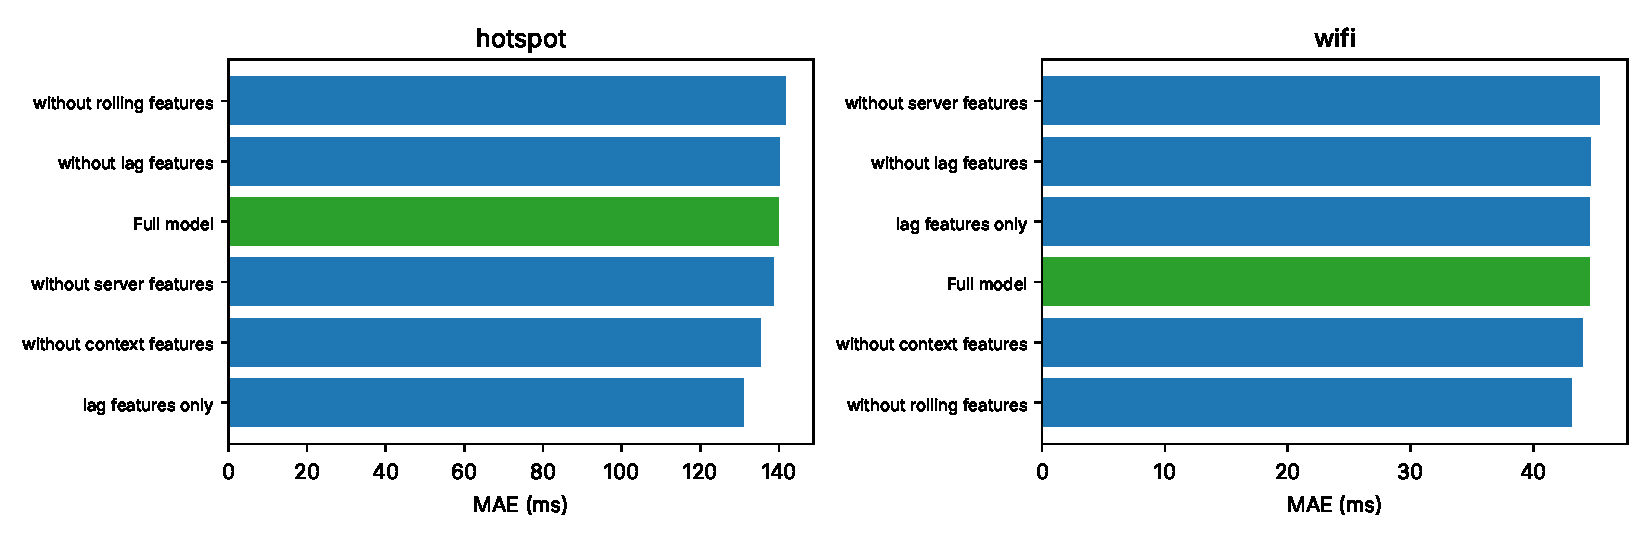
\includegraphics[width=\textwidth]{fig_ablation.pdf}
\caption{Ablation study: MAE of gradient boosting with different feature groups on the mobile hotspot (left) and Wi-Fi (right)}\label{fig:ablation}
\end{figure}

No feature group gave gradient boosting a clear benefit. With only the three lag features it was as accurate as the full model (44.56 ms in both cases), and removing the rolling statistics even lowered the MAE slightly, to 43.13 ms. Removing the server features caused the largest increase, to 45.40 ms, but all differences were smaller than the spread between test blocks. The Random Forest feature importances point the same way: the minimum of the last five RTTs dominated (\texttt{roll\_min5} (0.66), \texttt{srv\_median} (0.13), \texttt{roll\_mean12} (0.04), \texttt{srv\_code} (0.03), \texttt{lag1} (0.02), \texttt{ewma} (0.02)). The recent minimum is a robust estimate of the path's base delay (propagation plus transmission, Eq.~\ref{eq:delay}) that ignores short spikes, which also explains why smoothing methods do well. On the hotspot (Fig.~\ref{fig:ablation}), the lag-only model was the best variant (130.83 against 139.79 ms for the full model), so the extra features mainly added noise.

\subsection{Results under different conditions}\label{sec:conditions}

Table~\ref{tab:conditions} and Fig.~\ref{fig:horizon} show how the main models behave under three conditions: a longer prediction horizon, rounds with and without the background download, and a shorter training history (only the most recent part of each training set). The horizon and history experiments were run with the same forward-chaining design; the load comparison splits the main test predictions by the load flag.

\begin{table}[h]
\caption{MAE (ms) under different conditions (mean over 5 test blocks). The hotspot run had no background load}\label{tab:conditions}
\centering
\footnotesize
\begin{tabular}{@{}llcccc@{}}
\toprule
Condition & Level & Persistence & EWMA & Random Forest & Gradient boosting \\
\midrule
\multicolumn{6}{@{}l}{\textit{Wi-Fi}}\\
Horizon & 5 s & 50.61 & 41.37 & 41.57 & 44.56 \\
Horizon & 15 s & 51.58 & 42.32 & 40.61 & 43.33 \\
Horizon & 30 s & 53.43 & 43.18 & 40.77 & 43.86 \\
Horizon & 60 s & 51.76 & 42.71 & 39.41 & 43.39 \\
Background load & off & 51.81 & 42.11 & 42.19 & 44.99 \\
Background load & on & 48.26 & 39.92 & 40.34 & 43.70 \\
Training history & 10\% & -- & -- & 43.00 & 46.09 \\
Training history & 25\% & -- & -- & 41.41 & 46.88 \\
Training history & 50\% & -- & -- & 41.32 & 45.54 \\
\midrule
\multicolumn{6}{@{}l}{\textit{Mobile hotspot}}\\
Horizon & 5 s & 110.09 & 92.24 & 108.21 & 139.79 \\
Horizon & 15 s & 118.25 & 97.36 & 112.32 & 123.81 \\
Horizon & 30 s & 121.48 & 98.95 & 120.88 & 136.84 \\
Horizon & 60 s & 115.77 & 101.98 & 113.12 & 136.62 \\
Training history & 10\% & -- & -- & 93.03 & 107.43 \\
Training history & 25\% & -- & -- & 88.18 & 97.41 \\
Training history & 50\% & -- & -- & \textbf{85.00} & 92.69 \\
\botrule
\end{tabular}
\end{table}

\begin{figure}[h]
\centering
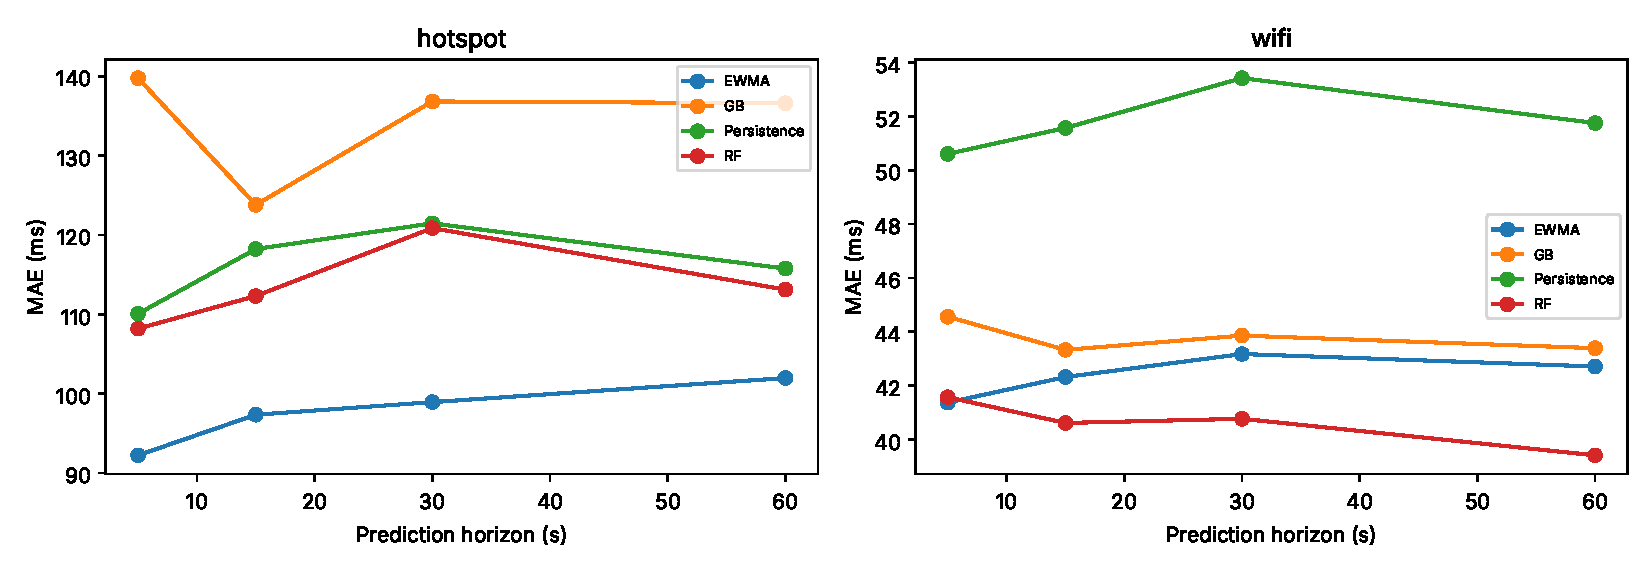
\includegraphics[width=\textwidth]{fig_horizon.pdf}
\caption{MAE for prediction horizons from 5 to 60 seconds on the mobile hotspot (left) and Wi-Fi (right)}\label{fig:horizon}
\end{figure}

Predicting further ahead hardly made the task harder: the MAE of EWMA rose only from 41.37 ms at 5 s to 42.71 ms at 60 s. Random Forest, however, improved with the horizon and was 7.7\% better than EWMA at 60 s (39.41 against 42.71 ms), which suggests that the learned models capture the typical level of each path better than its very next value. The background download did not make prediction harder; all models had slightly lower errors when it was on, consistent with the very small difference in median RTT reported in Table~\ref{tab:datasets}. Using only 10\% of the training history raised the MAE of Random Forest from 41.57 to 43.00 ms, so even a few minutes of recent data are enough to train a useful model. On the hotspot EWMA stayed best at every horizon, but the history experiment gave the most striking result: Random Forest trained on only the most recent half of each training set reached 85.00 ms, 8\% better than EWMA and 21\% better than the same model trained on all past data. The mobile path therefore changed during the run, and old measurements misled the learned models.

\subsection{Discussion}\label{sec:discussion}

The results answer the main question with a qualified \emph{it depends on the network}. On the stable Wi-Fi path, a machine-learning model that uses only information available on an end host predicted the next RTT significantly better than the EWMA estimator used in TCP, but the gain came from a simple linear model and was modest, 6.9\% in MAE, or about 2.9 ms. On the noisier mobile hotspot, no learned model beat EWMA, and the flexible models were much worse. Across both networks the Friedman ranks place ridge regression and EWMA level at the top, and the pre-declared gradient-boosting model near the bottom. Models with many parameters fit noise in the training data, and on a mobile path whose behaviour drifts within minutes, older training data actively hurt, as the training-history results show.

These findings connect to the literature in two ways. They support the long-standing use of EWMA in TCP \cite{jacobson1988,rfc6298}: it is hard to beat at short horizons and it adapts instantly to change. They also suggest that the larger gains reported for learned delay models \cite{rusek2020routenet,ferriol2023fermi,mostafavi2025delay} depend on information an ordinary host does not have, such as the network topology or radio conditions. For an application, the practical lesson is to use EWMA as the default, and to use a light linear model, retrained often on recent data only, where the path is stable.

The main threats to validity are the small number of networks and the short runs: one hour of Wi-Fi and 15 minutes of hotspot data from one laptop, with a background download that did not create measurable congestion. The results should therefore be read as a careful case study rather than a general claim about all networks.

% =====================================================================
%  Section 4: Conclusion
% =====================================================================
\section{Conclusion}\label{sec:conclusion}

This paper asked whether machine learning can predict the round-trip time of internet servers a few seconds ahead better than the simple estimators TCP already uses, using only information an ordinary end host has. To answer it, a measurement tool recorded the TCP handshake time to 12 servers in eight regions every 5 seconds, for one hour on a home Wi-Fi network and for 15 minutes on a mobile hotspot. Features were built only from past measurements, and eight predictors were compared with a forward-chaining evaluation in which every model was trained on the past and tested on the future, so no model could see future data.

The experiments support four conclusions. First, smoothing matters most: on Wi-Fi the EWMA estimator used in TCP reduced the error of simply repeating the last RTT from 50.61 ms to 41.37 ms. Second, on the stable Wi-Fi path a simple ridge regression was the most accurate model, with an MAE of 38.50 ms, 6.9\% lower than EWMA, a difference significant under both the Diebold--Mariano and Wilcoxon tests. Third, this gain did not transfer: on the mobile hotspot EWMA was the best method (92.24 ms) and every learned model was significantly worse, although Random Forest trained only on recent data beat it. Fourth, complex models did not help on either network; gradient boosting, chosen in advance as the proposed model, ranked near the bottom. In short, EWMA remains a strong default, and a light model gives only modest gains on stable paths.

\subsection{Limitations}\label{sec:limits}

\begin{itemize}
\item \textbf{Short runs from one laptop.} The data cover one hour of Wi-Fi and 15 minutes (173 rounds) of hotspot use, so the results may not hold for other networks, times of day or locations.
\item \textbf{No real congestion.} The background download barely changed the median RTT (99.5 against 101.1 ms), and the downloaded volume was not recorded, so the effect of heavy load on prediction was not tested.
\item \textbf{Handshake RTT only.} Measuring TCP handshakes to port 443 includes a small amount of server processing time, and content delivery networks may answer from different machines over time.
\item \textbf{Proposed model underperformed.} The gradient-boosting model chosen in advance was not the best; the winning ridge regression was identified by the experiment itself and should be confirmed on new data.
\item \textbf{Small test sets for significance.} Five test blocks and 12 servers give limited statistical power, and the Nemenyi test could not separate ridge regression from EWMA.
\end{itemize}

\subsection{Future work}\label{sec:future}

The next steps follow from these limitations. First, measurements should be repeated over several days and on other networks, such as campus networks and longer 4G or 5G runs, to see whether the ranking of models holds. Models retrained on a sliding window of recent data deserve particular attention, given their result on the hotspot. Second, the load generator should log its throughput and push the link to saturation, so that the effect of bufferbloat on prediction can be measured properly \cite{gettys2012bufferbloat,hoiland2016latency}. Third, the EWMA weight itself could be tuned online, and quantile models could predict the chance of a large spike rather than only the average RTT, which matters more for real-time applications. Finally, the best model could be built into a small client library that picks the fastest server or adjusts video quality, so that its benefit can be measured on real users.

\backmatter
\bmhead{Data and code availability}
The measurement tool (\texttt{collect\_latency.py}), the collected data and the analysis script (\texttt{latency\_ml.py}, random seed 42) reproduce every table and figure in Section~\ref{sec:results}.
\bibliography{references}

\subsection{Dataset and Implementation}

\textbf{Dataset:} The Wi-Fi and mobile-hotspot latency datasets were collected experimentally for this study, as described in Section~\ref{sec:datasets}. A public dataset URL is not currently available.

\textbf{Implementation:} The experiments were conducted using Python and scikit-learn. The source code used to generate the reported results is not currently available in a public GitHub repository.
\end{document}
